\subsubsection{Analytic \& Report}
\begin{figure}[H]
    \centering
    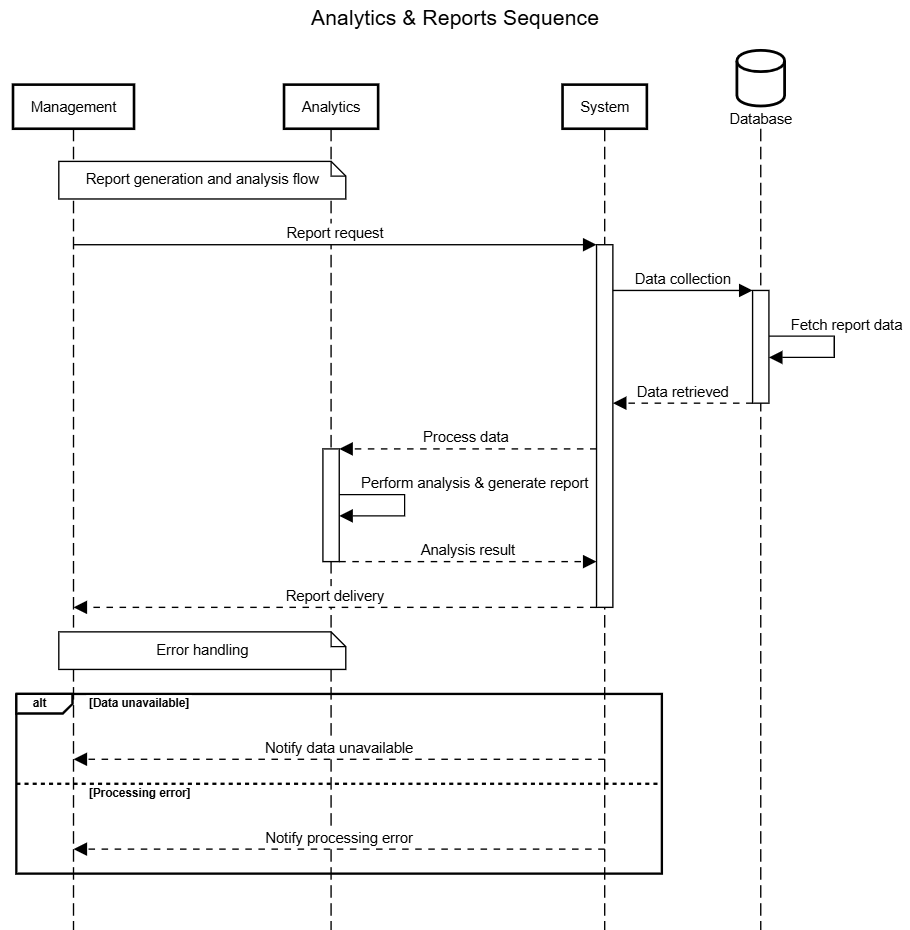
\includegraphics[width=0.8\textwidth]{graphics/chapter3/management/Analystic and Report.png}
    \caption{Sequence diagram of Analytics \& Report}
    \label{fig:search and book}
\end{figure}


\newpage
\noindent\textbf{Description}\\
\textbf{Actors:} Academic Affairs Office, Department Chair

\begin{enumerate}
    \item Management requests the System to generate a report.
    \item The System collects the required data from the Database.
    \item The System sends the collected data to the Analytics module for processing.
    \item The Analytics module analyzes the data and generates the analytical results.
    \item The Analytics module returns the analyzed results to the System.
    \item The System delivers the completed report to Management for review.
    \item If the necessary data is unavailable, the System notifies Management of the data unavailability.
    \item If an error occurs during processing, the System notifies Management of the processing error.
\end{enumerate}


